\documentclass[twoside]{jarticle}

\usepackage{grares}
\usepackage[dvipdfmx]{graphicx}
\usepackage{amsmath,amssymb}

\title{ターボ符号器における決定論的インタリーバの設計に関する研究}
\name{Bohulu Kwame Ackah}
\srnum{1631133}
\bib{}
\adviser{橋本 猛{情報伝送研究室}}
\date{\today}

\begin{document}
\MKTITLE

%%%%%%%%%%%%%%%%%%%%%%%%%%%%%%%%%%%%%%%%%%%%%%
\section{はじめに}
Claude Berrouにより提案されたターボ符号(TC)は、AWGNチャネルにおいて通信の容量を達成でき、誤り訂正符号の一つである。基本の場合、TCは、二つ以上の再帰的畳み込み符号(RSC符号)をインタリーバで並列連結して作られている。この2つのRSC符号は、要素符号と呼ばれる。TCのシステム図を図\ref{TC}に示す。
\begin{center}
\begin{figure}[h!]
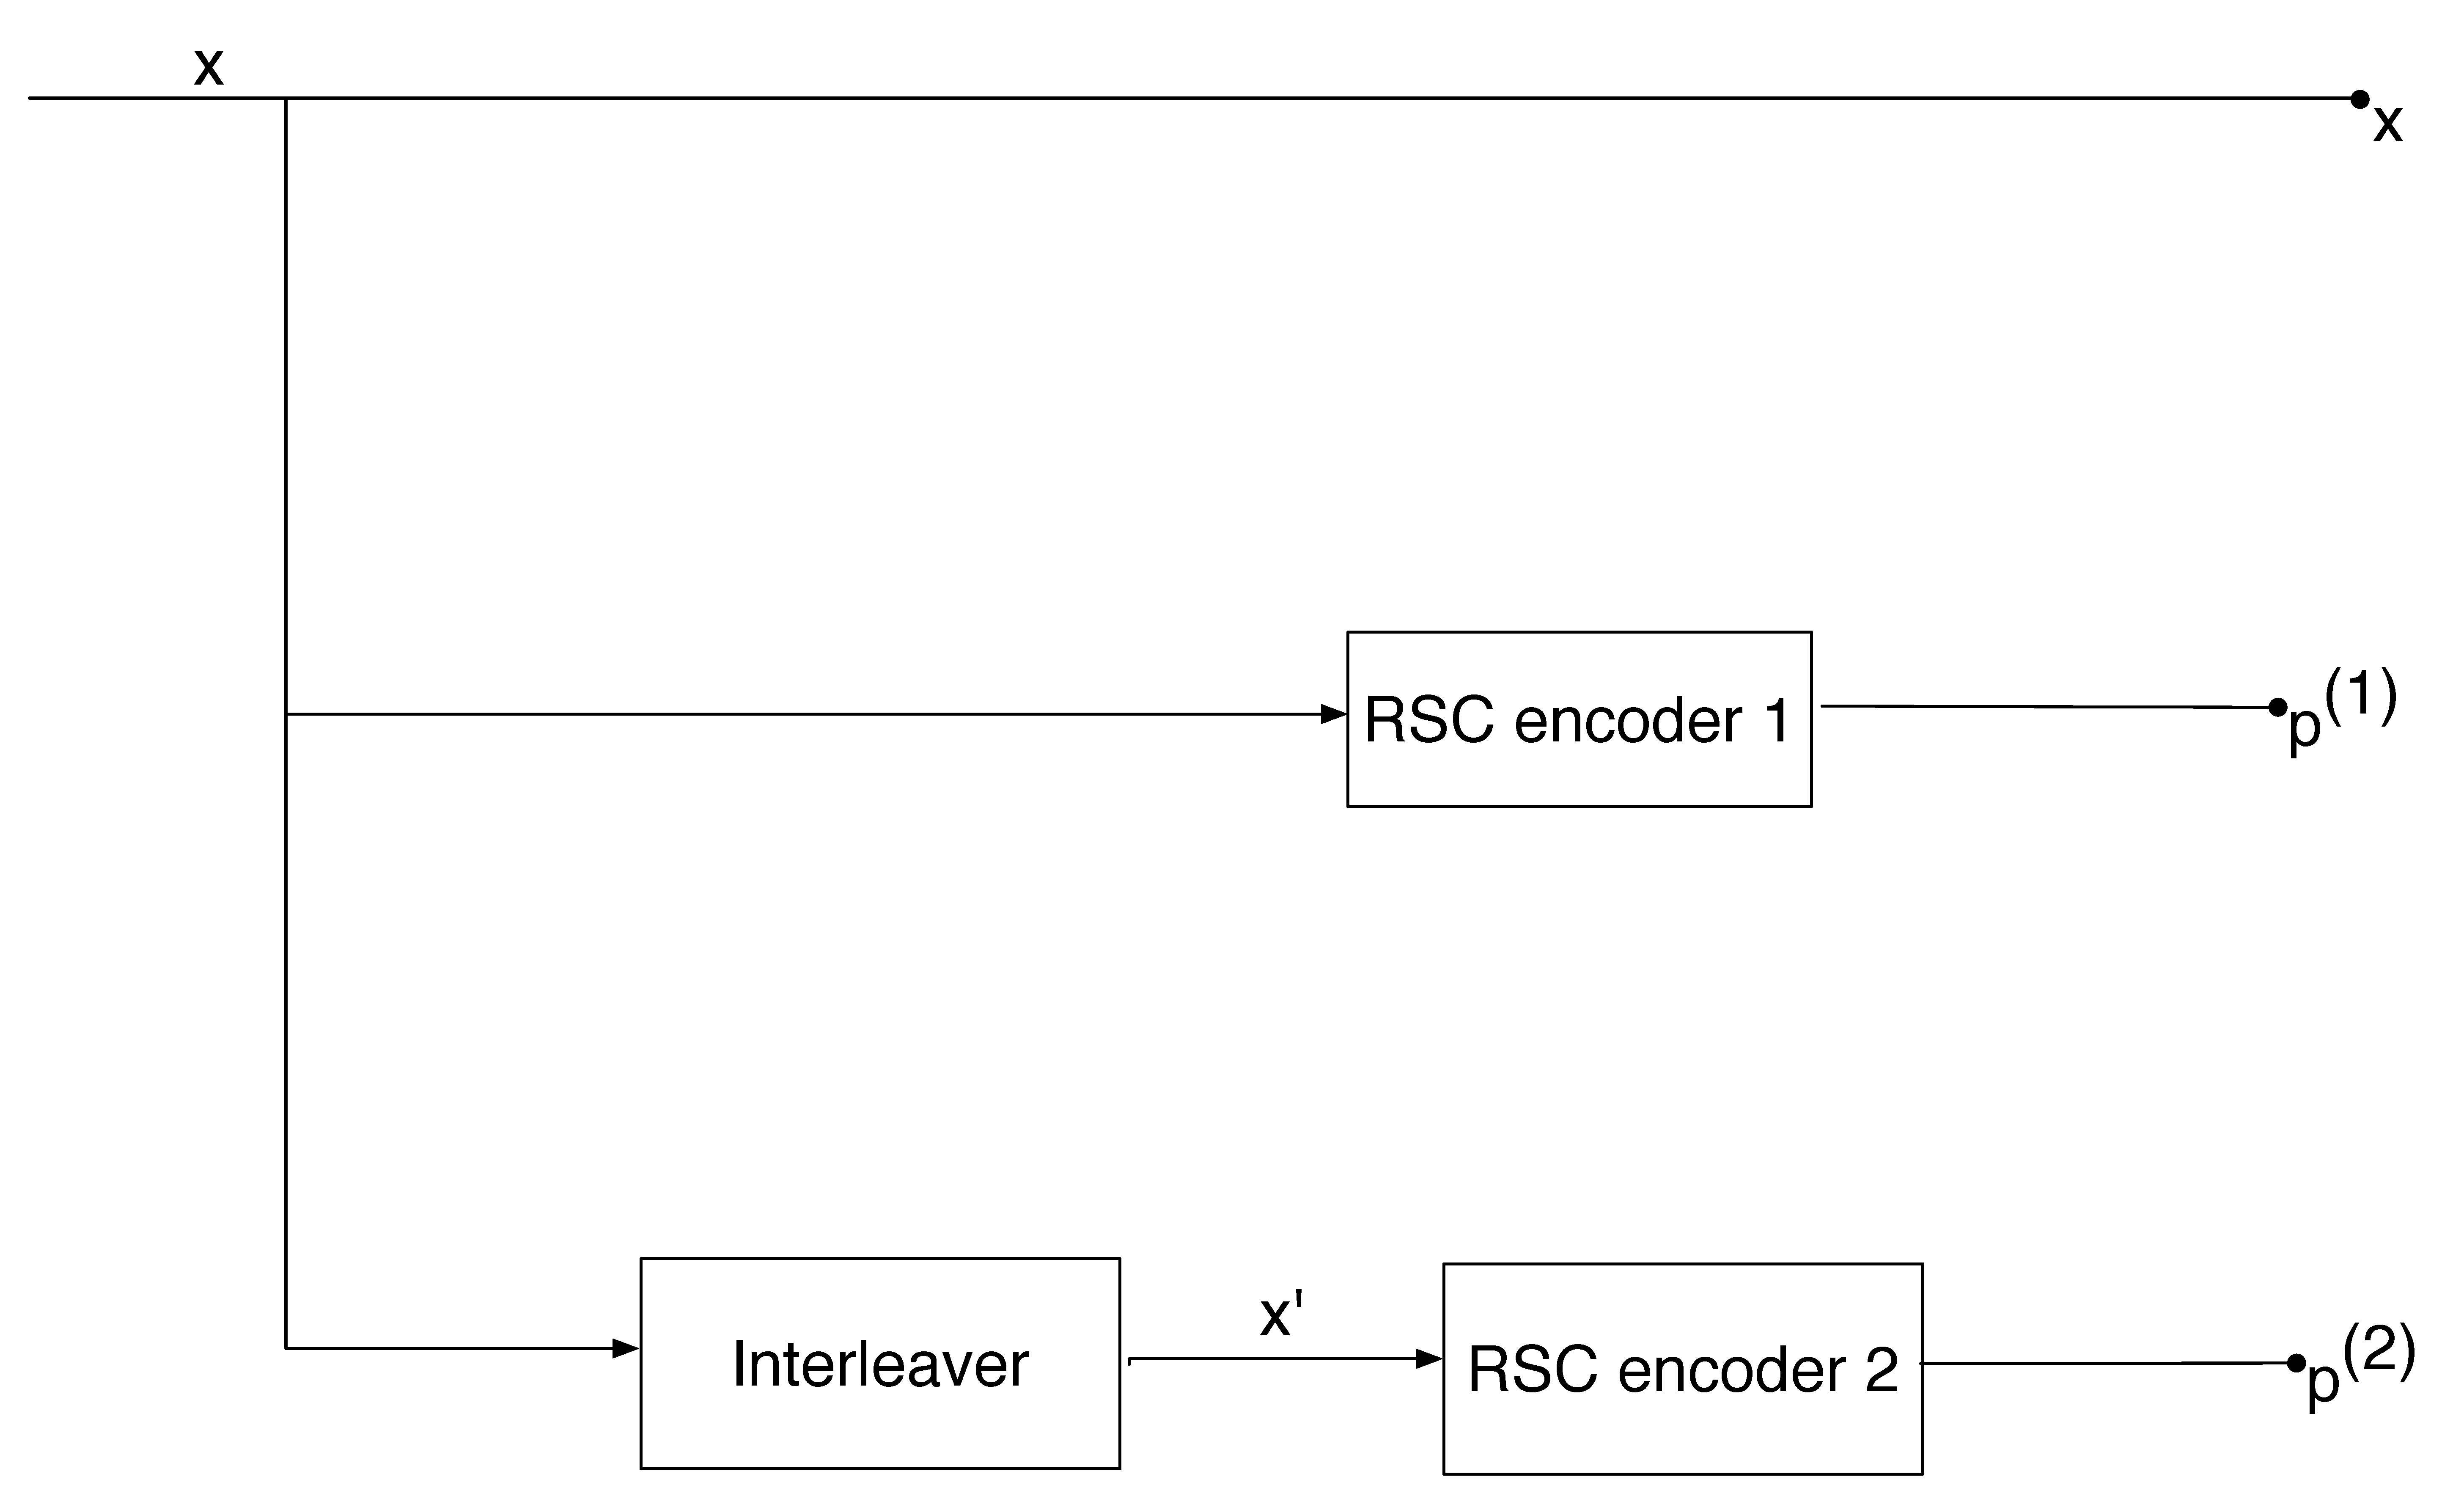
\includegraphics[width=6cm]{TurboEncoder.pdf}
\caption{ターボ符号器}
\label{TC}
\end{figure}
\end{center}
インタリーバは、ターボ符号の性能に大きな影響を与えるが、一般的に、ランダムインタリーバと決定論的いんたリーバの2つにグループ分けされている。

フレームサイズが長い場合、ランダムインタリーバは良い性能を持つが、TCは符号器と復号器にインタリーバテーブルを保存しなければならない。そのため、インタリーブとデインタリーブをアルゴリズムにより設計できる決定論インタリーバが、実用に多く採用されている。LTEでは、文献[3]で紹介されているPPIが採用されている。

フレームサイズが短い場合、決定論インタリーバはランダムインタリーバより良い性能を持つが、フレームサイズが長い場合、ランダムインタリーバより良い性能を持つ決定論インタリーバは、まだ見つかっていない。
本研究では、長いフレームサイズでランダムインタリーバより優れた決定論的インターリーバの開発を目標としている

%本研究では、フレームサイズが長い場合でも、ランダムインタリーバより良い性能を持つ決定論インタリーバを設計する。

%%%%%%%%%%%%%%%%%%%%%%%%%%%%%%%%%%%%%%%%%%%%%%
\section{システムモデル}
シミュレーションで使用するシステムモデルを図\ref{SystemModel}に示す。
\begin{center}
\begin{figure}[h!]
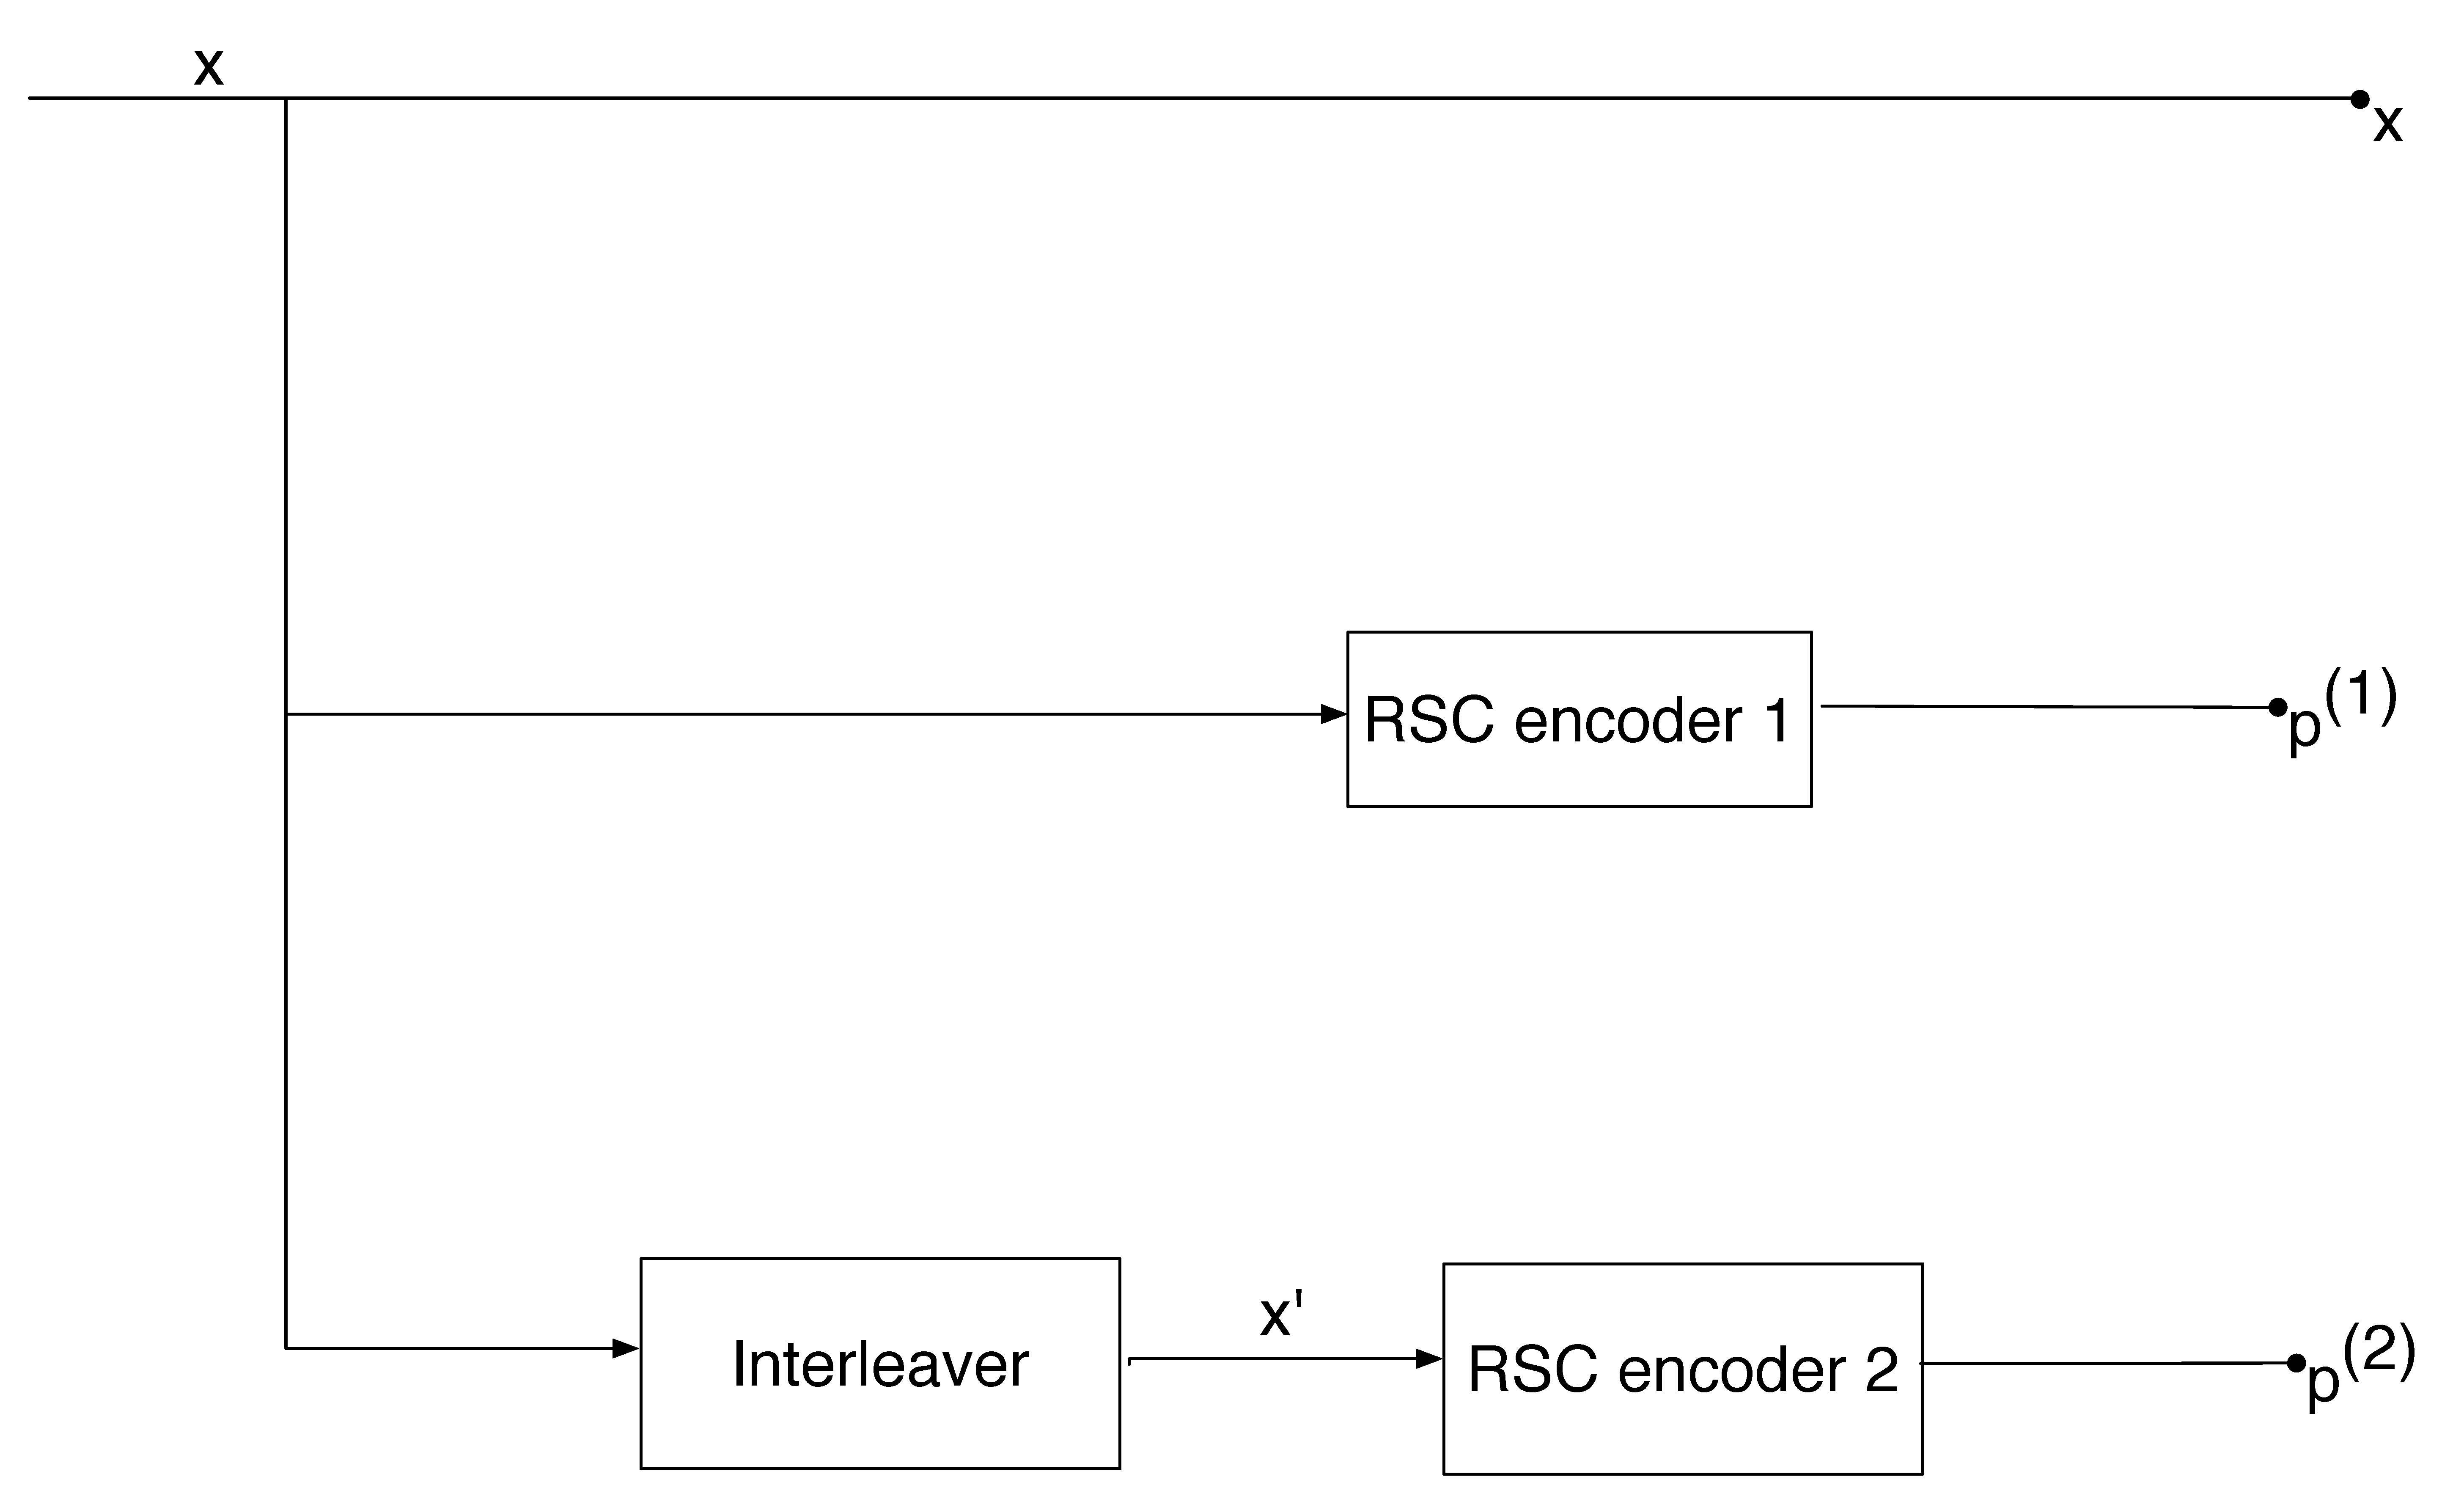
\includegraphics[width=6cm]{TurboEncoder.pdf}
\caption{システムモデル}
\label{SystemModel}
\end{figure}
\end{center}
長さ$N$の情報系列${\mbox{\boldmath$x$}}$をターボ符号器の1番目の要素符号(CE1)に入力し、インタリーバで並び替え、2番目の要素符号(CE2)に入力する。CE1とCE2 は同じRSC符号器である。次に、長さ$(n+1)N$のターボ符号器の出力${\mbox{\boldmath$x$}}$を、BPSK変調器に入力する。BPSK変調器は``$1$''を$1$に、``$0$''を$-1$に変調する。変調された出力$\widetilde{{\mbox{\boldmath$y$}}}$は加法性白色ガウス雑音(AWGN)通信路で送信され、AWGN通信路の出力$\widehat{{\mbox{\boldmath$y$}}}$をターボ復号器に入力する。ターボ復号器より長さ$N$の$\widehat{{\mbox{\boldmath$x$}}}$が出力され、ビット判定する。ここで、本資料で使用する記号を表1に示す。

\begin{center}
表1 使用する記号
 \begin{tabular}{||c c||} 
 \hline
 記号 & 意味\\ [0.5ex] 
 \hline\hline
 $x_i$ & i番目の情報ビットの位置  \\ 
 
  $d_{ef}$ &TCの有効自由距離  \\ 
  
   $\tau$ & RSC符号の周期  \\ 
 
 $n$ & 1ビットあたりの出力ビット  \\
 
 $K$ & 要素符号器の拘束長 \\
 
 $R$ & ターボ符号の出力レート \\
 
 $\tau$ &  要素符号器の周期長 \\
 
 $t$ & CE1でのタイプ1エラーイベントの長さ\\ 
 
  $s$ & CE2でのタイプ1エラーイベントの長さ\\ [1ex] 
 \hline
\end{tabular}
\end{center}

%%%%%%%%%%%%%%%%%%%%%%%%%%%%%%%%%%%%%%%%%%%%%%
\section{ターボ符号の性能解析}
\subsection{$a\tau$-2エラーイベント}
RSC符号は再帰的で、自由距離のプロパティが良いため、TCの設計にRSC符号を使用することは重要である。RSC符号器の周期長($\tau$)は一つの重要なパラメーターである。$\tau$は入力が[1, 0, 0, 0, ...]のときの出力の周期と定義される[3]。5/7 RSC符号器の場合、出力が[1, 1, 1, 0, 1, 1, 0, 1, 1, 0,....]である。周期は [1, 1, 0]で、$\tau$は3である。
入力系列のビット"1"を開始から$\tau$離れ、出力を合わせると符号語の重みが小さくなってしまう。

%SNRが高い場合、TCのビット誤り率(BER)性能は$d_{ef}$に依存することが先行研究で明らかにされている。$d_{ef}$とは、入力重み2エラーイベントが入力された場合のターボ符号語の最低距離である。

$a\tau$-2エラーイベントとは、$\tau$で離れたビット''1''二つを持つ情報系列である。
$$(1+D^{a\tau})(D^u)  \triangleq \mathbb{F}, 0\leq u\leq N-\tau, a=\{1,2,3,...\}$$
代表的な$a\tau$-2エラーイベントを図\ref{2m_error}に示す。ターボ符号にある重み2エラーイベントはそれぞれの要素符号にある$m$個の$a\tau$-2エラーイベントのことであり、インタリーバで繋がっている。
\begin{center}
\begin{figure}[h!]
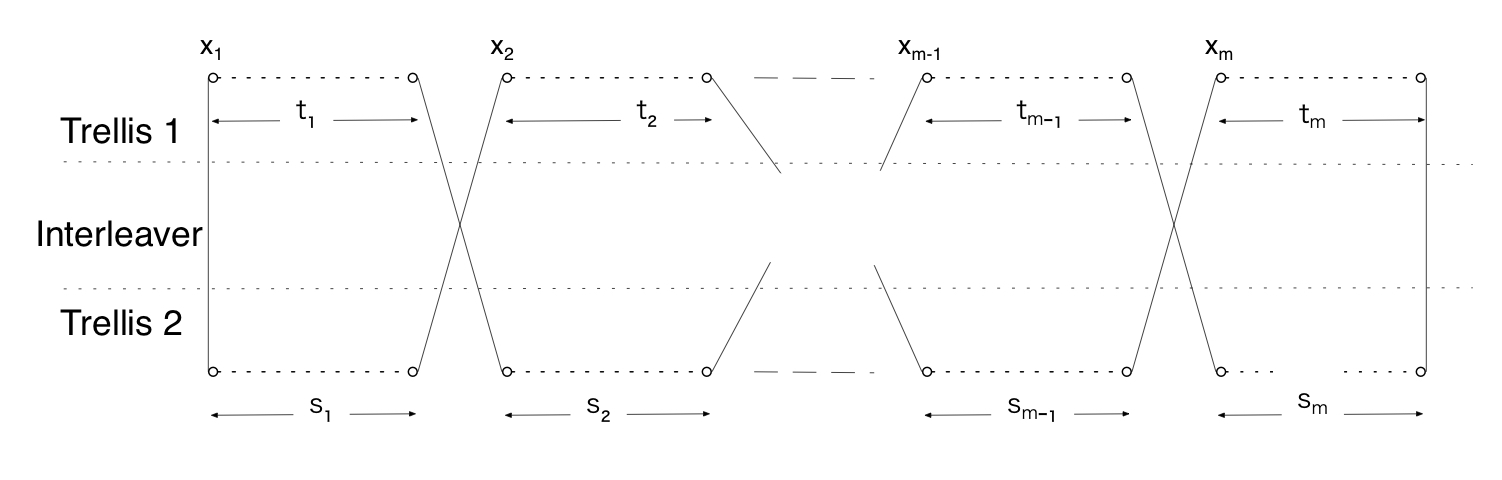
\includegraphics[width=8cm]{weight2m.jpg}
\caption{代表的な$a\tau$-2エラーイベント}
\label{2m_error}
\end{figure}
\end{center}
\vspace{-3mm}
CE1でのi番目の$a\tau$-2エラーイベントは長さ$t_i$を持ち、$x_i$から$x_i+t_i$まである。エラーイベントの開始と終了は$(x_i,x_i+t_i)$の整数組で表現されている。CE2でのi番目の$a\tau$-2エラーイベントは長さ$s_j$で、エラーイベントの開始と終了は$(x_i,x_i+s_j)$の整数組で表現されている。ターボ符号での$a\tau$-2エラーイベント葉整数組


\subsection{TCのビット誤り率性能}
TCに関する$a\tau$-2エラーイベントの符号語重みは、以下の式(\ref{dts})で計算できる[3]。
\begin{equation}
d_{(t_i,s_j)_v}=6m+\Bigg( \frac{ \left|t_i\right|}{\tau} + \frac{ \left|s_j\right|}{\tau} \Bigg)w_o
\label{dts}
\end{equation}

$1+D^\tau$の形を持つ入力系列の場合、$w_o$は1番目の要素符号の出力の重みである。

TCのBER性能の上界は式(\ref{Pb})で計算できる。

%設計されたインタリーバのマッピング関数は以下のように定義される。
%\begin{equation}
%\Pi(x_i) =[x_iD +\left \lfloor{x_i/A}\right \rfloor ]_N  %\[iD + \lfloor{\frac{i}{A}} \]\rfloor
%\end{equation}
%$$1 \leq D \leq L, C:=gcd(N,D), A:=N/C$$
%設計されたインタリーバを使用するターボ符号のビット誤り率性能を試さなくてはいけない。

%AWGN 通信路で最尤復号を使用した場合、畳み込み符号のBER性能は、upper bound technique上界できる[2]。

%\begin{equation}
%P_b \leq \sum_{i=1}^{2^N} \frac{w_i}{N}Q\Bigg( \sqrt{d_i\frac{2RE_b}{N_o}}\Bigg)
%\label{Pb}
%\end{equation}
 %$w_i$ と $d_i$は$i$番目の符号語の組織ビットの重みと合計ハミング重みである。
 
 %目的は$t+s$の最低値を大きくする$D$を見つけることである。

%$t$と$s$のすべての可能な値で、式(\ref{dts})で計算された同じ合計ハミング重みを持つ符号語が集められ、符号語あたりの平均組織ビット重みは以下のように定義する[1]。
%$W_d$は重み$d$を持つ符号語の合計組織ビットの重みで、そのため、式(\ref{Pb})を以下のように書き換えられる。
\begin{equation}
P_b \approx   \sum_{v=1}^{l} \frac{2mN_{d_{(t_i,s_j)_v}}}{N}Q\Bigg( \sqrt{d_{(t_i,s_j)_v}\frac{2RE_b}{N_o}}\Bigg)
\label{Pb}
\end{equation}
ここで、 $N_{d_{(t_i,s_j)_v}}$は重み$d_{(t_i,s_j)_v}$を持つ符号語の数であり、$l$は$(1+D^{a\tau})(D^u) ,0\leq u\leq N-\tau, a=\{1,2,3\}$の形を持つ入力重み2mエラーイベントの合計数である。
%$$l=\sum_{a=1}^{3}N-(N-a\tau)$$である。
$m=1$で、$t_i=s_j$の場合、以下の図\ref{2_error}を使用してインタリーバの設計考える。
\begin{center}
\begin{figure}[h!]
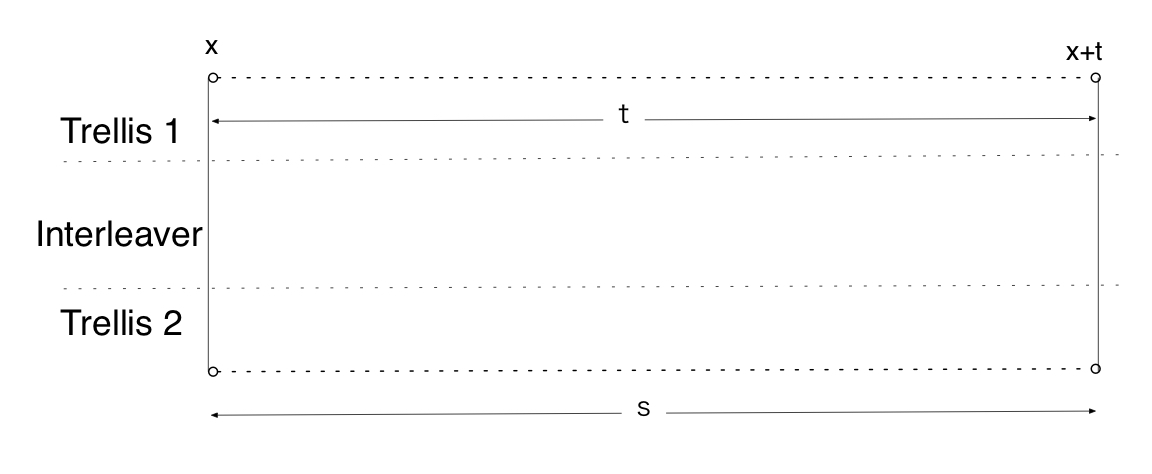
\includegraphics[width=8cm]{weight2.jpg}
\caption{$t=s=\tau$のエラーイベント}
\label{2_error}
\end{figure}
\end{center}
図\ref{2_error}はTCの$d_{ef}$に関するからである。$d_{ef}$とは、入力重み2エラーイベントが入力された場合のターボ符号語の最低距離である。
\vspace{-3mm}
%%%%%%%%%%%%%%%%%%%%%%%%%%%%%%%%%%%%%%%%%%%%
\section{線形インタリーバの最適化}



%$(1+D^{a\tau})(D^u) ,0\leq u\leq N-\tau$の形を持つ入力重み2エラーイベント(タイプ1エラーイベント)をRSC符号に入力する場合、低い重みをもつ符号語を作成できることが、先行研究で明らかになった。
TCの$d_{ef}$を大きくするために、
%$$s \leq a\tau \triangleq \mathbb{E}(s) \\\\\ \forall x \in \mathbb{Z} , t \in \mathbb{D}$$
$t = s =\tau$を防ぐようなインタリーバを設計する必要がある。線形インタリーバのマッピング関数は式(\ref{linear})で定義される[1]。
\begin{equation}
\Pi_{\mathbf{L}_n}(i) \equiv bi  \mod N, \ 0 \leq i \leq N
\label{linear}
\end{equation}
bは、Nとお互いにそう整数である。式(\ref{dts})を大きくするdは以下の方法で検索する。

%言い換えると、TCの$d_{ef}$値を大きくするために、$t+s$をより大きくできるインタリーバが望ましい。

%%%%%%%%%%%%%%%%%%%%%%%%%%%%%%%%%%%%%%%%%%%%%%
\subsection{bの検索方法}
bのすべての可能な値で、$\Pi_{\mathbf{L}_n}(i+t)-\Pi_{\mathbf{L}_n}(i)=s$を計算する。式\ref{dts}で$d_{(t_i,s_j)_v}$を計算してmin $d_{(t_i,s_j)_v}$を選ぶ。最後に、bに関するmax(min $d_{(t_i,s_j)_v}$)を選択する。
\vspace{-3mm}
%%%%%%%%%%%%%%%%%%%%%%%%%%%%%%%%%%%%%%%%%%%%%%
\begin{thebibliography}{}
  \bibitem{1}  Oscar Y. Takeshita, Member, IEEE, and Daniel J. Costello ,''New Deterministic Interleaver Designs for Turbo Codes'',IEEE Trans. Inform. Theory, vol. 46,pp. 1988-2006,Nov. 2000\\
  \bibitem{2} L. C. Perez, J. Seghers, D. J. Costello, Jr., ''A distance spectrum interpretation of turbo codes'', IEEE Trans. Inform. Theory, vol. 42, pp. 1698-1709, Nov. 1996.\\
\bibitem{3} Jing Sun, Oscar Y. Takeshita ”Interleavers for Turbo Codes Using Permutation Polynomials over Integer Rings”, IEEE Trans. Inform. Theory, vol. 51,
pp. 101 - 119 Jan. 2005\\
\bibitem{4} John G. Proakis, Masoud Salehi. ''Digital Communications'', Fifth Edition,Chapter 8, McGraw-Hill\\.
\end{thebibliography}



\end{document}
